\chapter{Data Driven Surrogate Signal Extraction for Dynamic PET} \label{sec:data_driven_surrogate_signal_extraction_results}
            
    
    \longsection{PCA Data Driven Surrogate Signal Extraction Methods for Dynamic PET}{sec:pca_data_driven_surrogate_signal_extraction_methods_for_Dynamic_pet}
        Respiratory motion correction is beneficial in positron emission tomography. Methods of motion correction include gated reconstruction where the acquisition is binned based on a respiratory trace. To acquire these respiratory traces an external device like the Real Time Position Management system or a data driven method such as principal component analysis can be used. Data driven methods have the advantage that they are non-invasive and can be performed post-acquisition. However, data driven methods have the disadvantage that they are adversely affected by the tracer kinetics of a dynamic acquisition. This work seeks to evaluate several adaptions of the principal component analysis method through which it  can be used with dynamic data. The methods explored in this work include using a moving window, and re-use of the principal component from a later time frames to estimate the surrogate signal from earlier data. The respiratory traces acquired were evaluated by calculating their cross correlation with a Real Time Position Management surrogate signal and also by performing and comparing gated reconstructions using the traces. The results indicate that all methods produce better surrogate signals than when applying static PCA to dynamic data. Re-using a late principal component for the start of the scan produced the most promising results. Future research includes further tuning the hyper parameters, evaluating the methods on a larger set of data, and using the extract respiratory signal in more complex motion correction algorithms for dynamic PET.
        
        \subsection{Introduction} \label{sec:pca_data_driven_surrogate_signal_extraction_methods_for_Dynamic_pet_introduction}
            Respiratory motion reduces image resolution in \gls{PET} by introducing blurring and mis-alignment artefacts~\cite{Nehmeh2008a}. This is often combated through the use of gated reconstruction and motion correction, potentially as a first step towards obtaining motion corrected images. Gating requires a \gls{SS} which reflects the position in which the internal organs are in the respiratory cycle. Methods to determine \glss{SS} include those which use an external devices, like the \gls{RPM}. However, a disadvantage of these methods are that they require the use of additional equipment and a change to clinical practise. Thus, \gls{DD} methods to extract \glss{SS} have become an alternative, these include \gls{PCA}~\cite{Thielemans2011}. To the best of our knowledge, current \gls{DD} \gls{SS} extraction methods fail for dynamic \gls{PET} data where the tracer kinetics, at the start of the acquisition, offer more variance than the respiratory motion does. Previously, a moving window based approach using the spectral analysis method was proposed~\cite{Schleyer2014}. This work seeks to implement a moving window method using \gls{PCA} and then compare this to static \gls{PCA} and other \gls{PCA} based dynamic \gls{DD} \gls{SS} extraction methods.
        
        \subsection{Methods} \label{sec:pca_data_driven_surrogate_signal_extraction_methods_for_Dynamic_pet_methods}
            \subsection{Data Acquisition} \label{sec:pca_data_driven_surrogate_signal_extraction_methods_for_Dynamic_pet_data_acquisition}
                Five dynamic \gls{FDG} acquisitions, with a \gls{FOV} covering the upper lung and heart, were acquired on a \gls{GE} Discovery $710$. Each acquisition lasted approximately \SI{20}{\minute} with the acquisition starting before injection of the radiotracer. \glss{SS} were acquired in parallel using a \gls{RPM}.
                
            \subsection{Data Preparation} \label{sec:pca_data_driven_surrogate_signal_extraction_methods_for_Dynamic_pet_data_preparation}
                Data were unlisted into low resolution sinograms, at a time interval of \SI{500}{\milli\second}, using the \gls{GE} PetToolbox following~\cite{Bertolli2018Data-DrivenTomography}. Data was preprocessed by removing the first and last sinogram in the axial direction and applying a Freeman-Tukey transformation to stabilise the variance of the Poisson data \cite{Freeman1950TransformationsRoot}. The Freeman-Tukey transformation is defined as:

                \begin{equation}
                    S_g := 2 \sqrt{S_p + \frac{3}{8}}
                \end{equation}

                \noindent $S_g$ is the resultant, Gaussian distributed, sinogram of applying the Freeman-Tukey transformation to Poisson distributed sinogram $S_p$~\cite{Freeman1950TransformationsRoot}.
            
            \subsection{Surrogate Signal Extraction} \label{sec:surrogate_signal_extraction}
                In a first attempt static \gls{PCA} was applied to the entire acquisition. This was compared with:
                
                \subsubsection{Moving Window} \label{sec:pca_data_driven_surrogate_signal_extraction_methods_for_Dynamic_pet_moving_window}
                    This method takes data window by window (with half a window overlap) and extracts a \gls{SS} using \gls{PCA}. The final \gls{SS} is constructed by determining the sign of the current \gls{SS} (using \gls{CC} in the overlap with the previous window), flipping it if necessary, and then, taking the mean where it overlaps, and concatenating it with the previous \gls{SS}. The size of the window increases as the acquisition goes on. The motivation is that at early time points the variation caused by the tracer kinetics obscures that which comes from respiratory motion, and reducing the window size decreases the change in the data due to the tracer kinetics.
                
                \subsubsection{One \gls{PC}} \label{sec:pca_data_driven_surrogate_signal_extraction_methods_for_Dynamic_pet_one_pc}
                    This method takes a late time point \gls{PC} and applies it to early time point data using the normal formula to find the weight at a particular time point. The motivation is that the \glss{PC} of late time point data capture mostly the respiratory motion only. This was verified by checking that the late time point \glss{PC} did not vary substantially.
            
            \subsection{Evaluation} \label{sec:pca_data_driven_surrogate_signal_extraction_methods_for_Dynamic_pet_evaluation}
                \subsubsection{Cross Correlation} \label{sec:pca_data_driven_surrogate_signal_extraction_methods_for_Dynamic_pet_cross_correlation}
                    The \gls{CC} of each \gls{SS} between each method and the \gls{RPM}, for all acquisitions, has been calculated. Additionally, the early time point \glss{SS} for each method have been plotted against the \gls{RPM}, for the first acquisition.
                
                \subsubsection{Reconstruction} \label{sec:pca_data_driven_surrogate_signal_extraction_methods_for_Dynamic_pet_reconstruction}
                    Data has been reconstructed, for the first acquisition, using each \gls{SS} to displacement gate the data into $10$ bins. Reconstructions were performed using \gls{GE} Duetto with \gls{TOF} \gls{OSEM} using two full iterations and $24$ subsets~\cite{Hudson1994}.
                    Attenuation, scatter and randoms were not taken into account. Volumes were post-filtered using a Gaussian blur with a kernel size of \SI{6.4}{\milli\metre} \gls{FWHM}.
                    
                    Comparisons between these motion corrected reconstructed volumes includes: A profile over the aorta and \gls{SUV}\textsubscript{max}, \gls{SUV}\textsubscript{median} and \gls{SUV}\textsubscript{peak}. \gls{SUV}\textsubscript{peak} here was defined following \gls{EANM} guidelines~\cite{Boellaard2015FDG2.0}
            
        \subsection{Results} \label{sec:pca_data_driven_surrogate_signal_extraction_methods_for_Dynamic_pet_results}
            \begin{table}
                \centering
                
                \captionsetup{singlelinecheck=false, justification=centering}
                \caption{A comparison of the \gls{CC} between the \gls{RPM} \gls{SS} and the \gls{SS} from the static \gls{PCA}, the moving window and the one \gls{PC} method for five acquisitions.}
                
                \resizebox*{1.0\linewidth}{!}
                {
                    \begin{tabular}{||c|ccc||}
                        \hline
                        \textbf{\gls{CC}} & \textbf{Static \gls{PCA}} & \textbf{Moving Window} & \textbf{One \gls{PC}} \\
                        \hline
                        \textbf{Acquisition one}    & $0.0412$  & $0.670$ & $0.851$ \\
                        \textbf{Acquisition two}    & $0.0269$  & $0.582$ & $0.901$ \\
                        \textbf{Acquisition three}  & $0.00579$ & $0.804$ & $0.869$ \\
                        \textbf{Acquisition four}   & $0.0321$  & $0.714$ & $0.859$ \\
                        \textbf{Acquisition five}   & $0.0220$  & $0.596$ & $0.779$ \\
                        \hline
                    \end{tabular}
                }
                \label{tab:pca_data_driven_surrogate_signal_extraction_methods_for_Dynamic_pet_cross_correlation}
            \end{table}
            
            A comparison of \gls{CC} can be seen in~\Fref{tab:pca_data_driven_surrogate_signal_extraction_methods_for_Dynamic_pet_cross_correlation}. The results for both the moving window and the one \gls{PC} method show that they perform better than static \gls{PCA}. The results for the moving window method are more varied than the one \gls{PC} method as it has far more hyper parameters and is substantially more sensitive to them.
            
            \begin{figure}
                \centering
                
                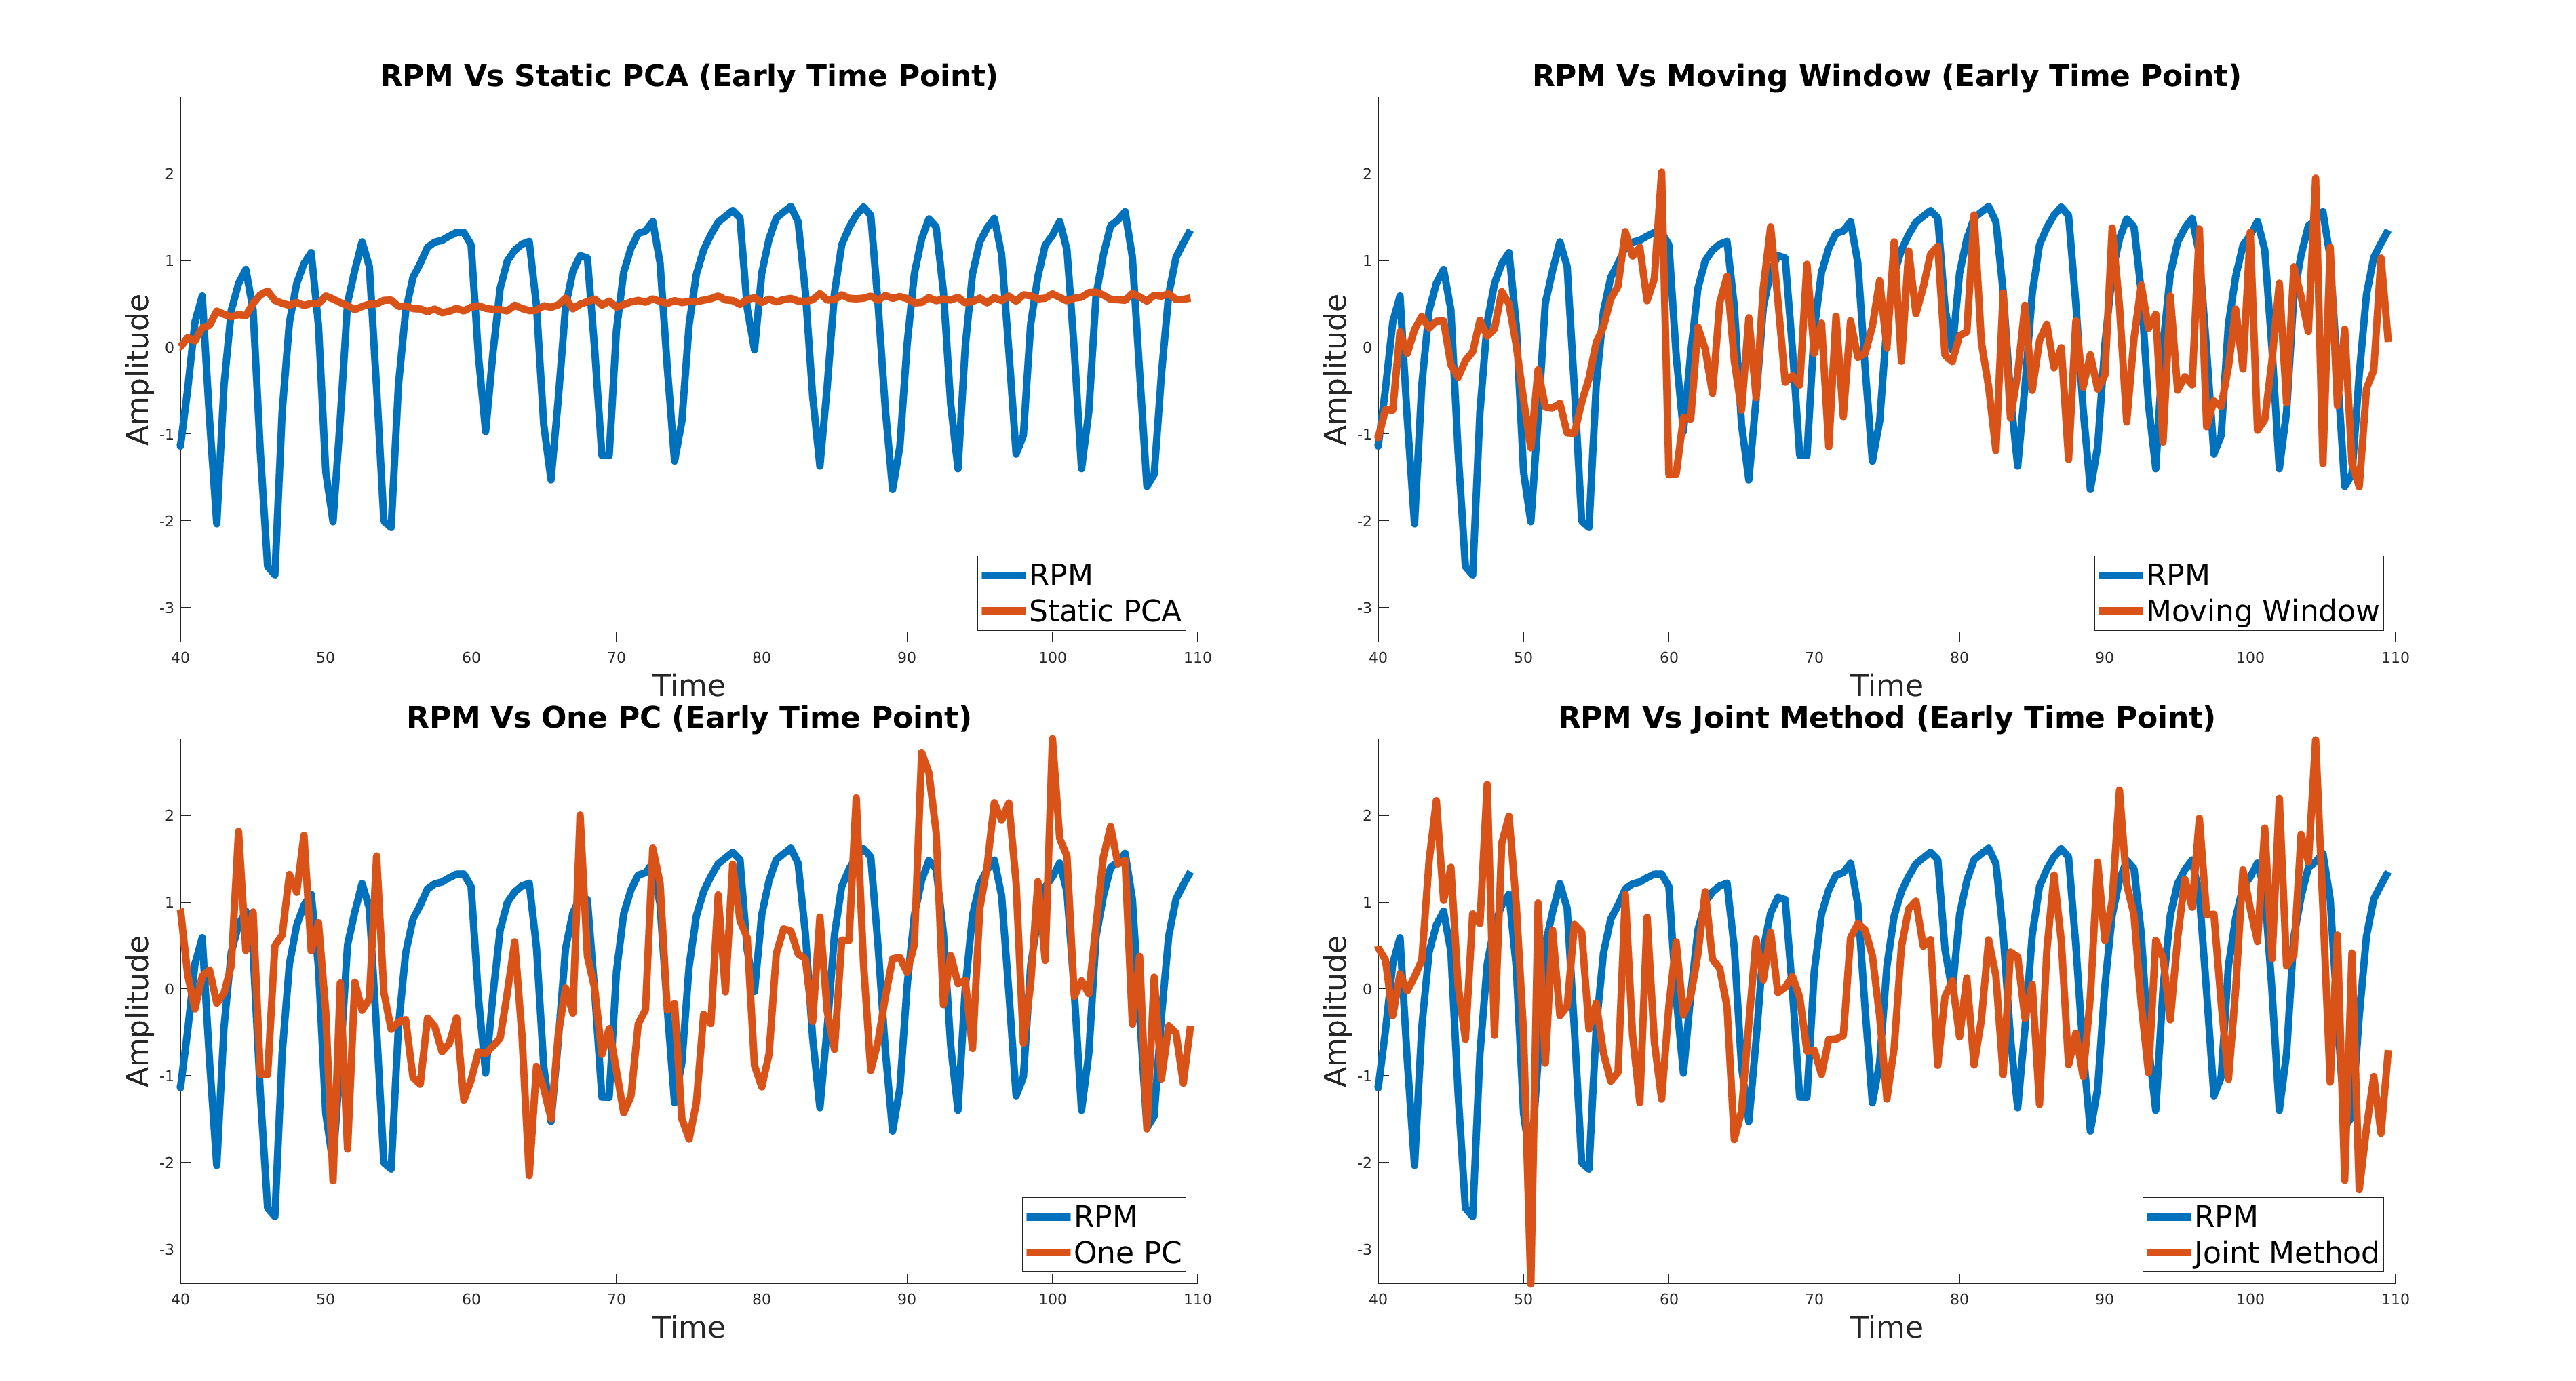
\includegraphics[width=1.0\linewidth]{figures/data_driven_surrogate_signal_extraction_results_1_surrogate_signal.png}
                
                \captionsetup{singlelinecheck=false, justification=centering}
                \caption{A visual comparison between the \gls{RPM} \gls{SS} and the \gls{SS} from the static \gls{PCA}, the moving window and the one \gls{PC} for acquisition one between \SI{40}{\second} and \SI{110}{\second}.}
                \label{fig:pca_data_driven_surrogate_signal_extraction_methods_for_Dynamic_pet_surrogate_signal}
            \end{figure}
            
            \begin{figure}
                \centering
                
                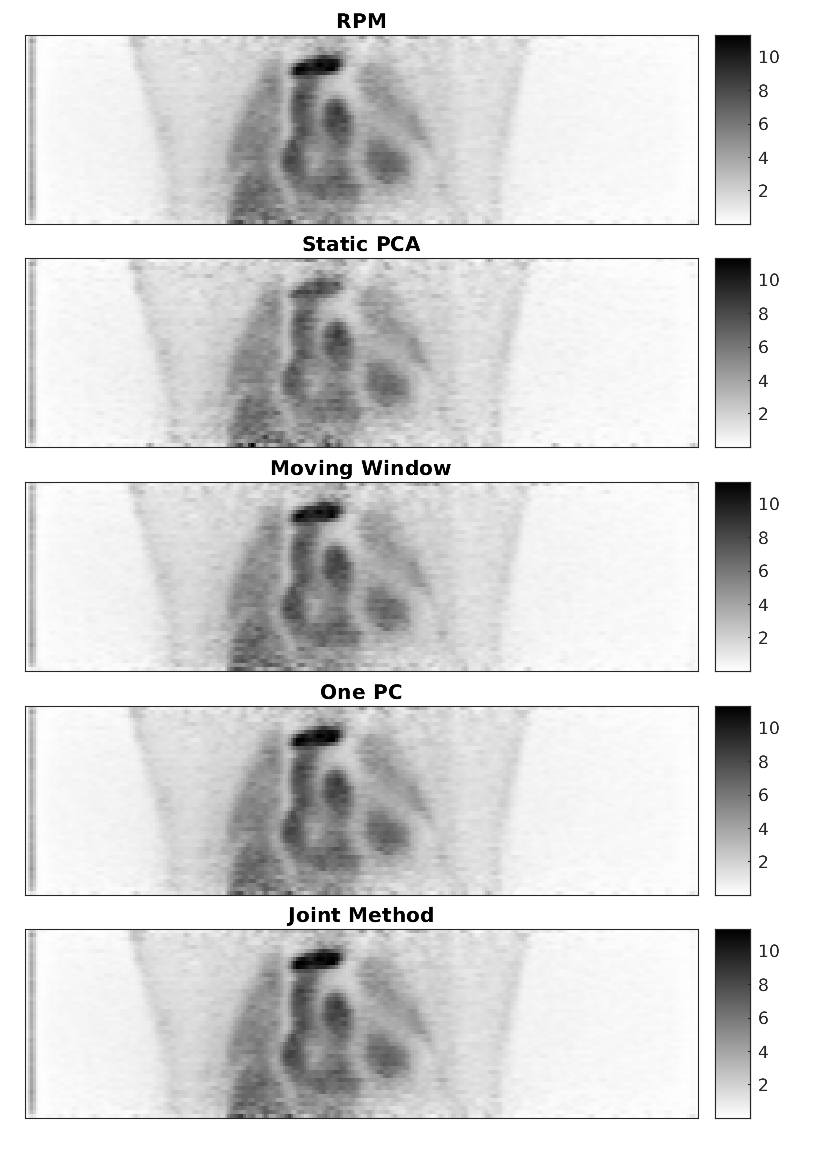
\includegraphics[width=0.8\linewidth]{figures/data_driven_surrogate_signal_extraction_results_1_visual_analysis_pca.png}
                
                \captionsetup{singlelinecheck=false, justification=centering}
                \caption{Gated reconstructions of acquisition one using the \gls{RPM}, static \gls{PCA}, moving window and one \gls{PC} method \gls{SS}. Colour map ranges are consistent for all images.}
                \label{fig:pca_data_driven_surrogate_signal_extraction_methods_for_Dynamic_pet_visual_analysis}
            \end{figure}
            
            \begin{figure}
                \centering
                
                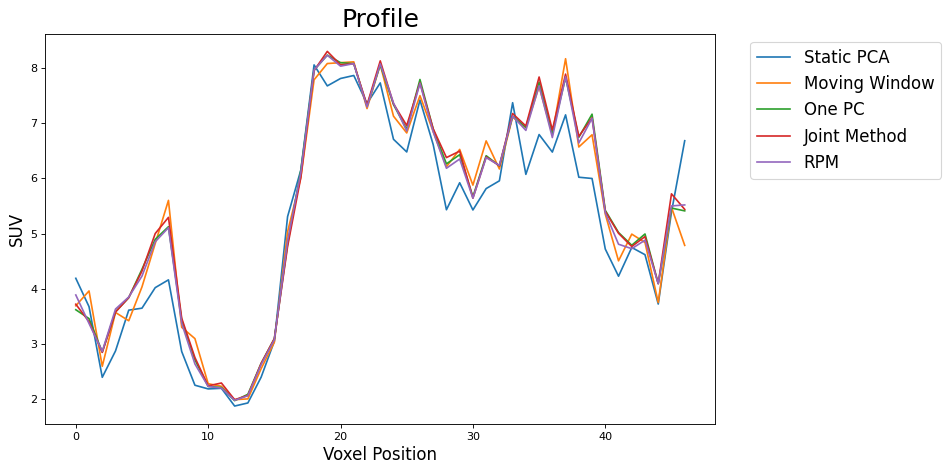
\includegraphics[width=1.0\linewidth]{figures/data_driven_surrogate_signal_extraction_results_1_profile_pca.png}
                
                \captionsetup{singlelinecheck=false, justification=centering}
                \caption{A profile across the aorta, in the superior-inferior direction, for gated reconstructions of acquisition one using the \gls{RPM}, static \gls{PCA}, moving window and one \gls{PC} method \gls{SS}.}
                \label{fig:pca_data_driven_surrogate_signal_extraction_methods_for_Dynamic_pet_profile}
            \end{figure}
            
            \begin{table}
                \centering
                
                \captionsetup{singlelinecheck=false, justification=centering}
                \caption{Comparison of \gls{SUV}\textsubscript{max}, \gls{SUV}\textsubscript{median} and \gls{SUV}\textsubscript{peak} between gated reconstructions of acquisition one using the \gls{RPM}, static \gls{PCA}, moving window and one \gls{PC} method \gls{SS}.}
                
                \resizebox*{0.75\linewidth}{!}
                {
                    \begin{tabular}{||c|ccc||}
                        \hline
                        \textbf{\gls{SUV}} & \textbf{Max} & \textbf{Median} & \textbf{Peak} \\
                        \hline
                        \textbf{\gls{RPM}}          & $18.4$ & $10.9$ & $12.6$ \\
                        \hline
                        \textbf{Static \gls{PCA}}   & $12.8$ & $10.6$ & $11.4$ \\
                        \textbf{Moving Window}      & $14.5$ & $10.6$ & $11.3$ \\
                        \textbf{One \gls{PC}}       & $18.5$ & $10.9$ & $12.6$ \\
                        \hline
                    \end{tabular}
                }
                \label{tab:pca_data_driven_surrogate_signal_extraction_methods_for_Dynamic_pet_suv}
            \end{table}
            
            A plot of the \gls{SS} for all methods can be seen in~\Fref{fig:pca_data_driven_surrogate_signal_extraction_methods_for_Dynamic_pet_surrogate_signal}, the one \gls{PC} method matches the \gls{RPM} best in this example. The reconstructed data, using \glss{SS} from all methods can be seen in~\Fref{fig:pca_data_driven_surrogate_signal_extraction_methods_for_Dynamic_pet_visual_analysis}, the clarity of the reconstruction around the aorta seems diminished in the static \gls{PCA} example, it is similar in all other examples. A profile across the aorta can be seen in~\Fref{fig:pca_data_driven_surrogate_signal_extraction_methods_for_Dynamic_pet_profile}, this shows that the static \gls{PCA} method differs in its distribution. \gls{SUV} results can be seen in~\Fref{tab:pca_data_driven_surrogate_signal_extraction_methods_for_Dynamic_pet_suv} and show that \glss{SUV} are consistent with \gls{RPM} for both the one \gls{PC} method.
            
        \subsection{Discussion and Conclusion} \label{sec:pca_data_driven_surrogate_signal_extraction_methods_for_Dynamic_pet_discussion_and_conclusion}
            Results from a comparison of \gls{CC}, profiles and \glss{SUV} show that the moving window and one \gls{PC} show promise in \gls{DD} extraction of \gls{SS} from dynamic data when compared to the static method.
            
            In the future, research will focus on further development of the one \gls{PC} method, including tuning its hyper parameters as well as testing it on a wider array of data.
    
%    \longsection{Feasibility Study of Neural Network Based Data Driven Surrogate Signal Extraction Methods for Dynamic PET}{sec:feasibility_study_of_neural_network_based_data_driven_surrogate_signal_extraction_methods_for_dynamic_pet}
        
        
%        \subsection{Introduction} \label{sec:feasibility_study_of_neural_network_based_data_driven_surrogate_signal_extraction_methods_for_dynamic_pet_introduction}
            
        
%        \subsection{Methods} \label{sec:feasibility_study_of_neural_network_based_data_driven_surrogate_signal_extraction_methods_for_dynamic_pet_methods}
            
            
%        \subsection{Results} \label{sec:feasibility_study_of_neural_network_based_data_driven_surrogate_signal_extraction_methods_for_dynamic_pet_results}
            
            
%        \subsection{Discussion and Conclusion} \label{sec:feasibility_study_of_neural_network_based_data_driven_surrogate_signal_extraction_methods_for_dynamic_pet_discussion_and_conclusion}
            
